\documentclass{beamer}

\usepackage{beamerthemesplit}
\usepackage{verbatim}
\usepackage[normalem]{ulem}

\usepackage{xcolor}

\usepackage{hyperref}

\definecolor{gold}{rgb}{1.,0.84,0.}
\definecolor{brightred}{rgb}{1.,0.4,0.4}
\definecolor{mygray}{RGB}{200,200,200}
\definecolor{lightsteelblue}{RGB}{176,196,222}
\definecolor{lightskyblue}{RGB}{135,206,250}
\definecolor{cadetblue}{RGB}{95,158,160}

\usetheme{default}
\usecolortheme{mule}

\usefonttheme{serif}

%\DeclareGraphicsExtensions{.pdf,.png,.jpg}

\newcommand{\snr}{$S/N$}
\newcommand{\snT}{$(S/N)_{\textrm{size}}$}
%\newcommand{\snT}{$\left( \frac{S}{N}\right)_{\textrm{size}}$}
\newcommand{\snflux}{$(S/N)_{\textrm{flux}}$}
%\newcommand{\snflux}{$\left( \frac{S}{N}\right)_{\textrm{flux}}$}

\newcommand{\lensfit}{\texttt{LENSFIT}}
\newcommand{\numba}{\texttt{Numba}}
\newcommand{\python}{\texttt{Python}}
\newcommand{\ngmix}{\texttt{ngmix}}
\newcommand{\shear}{{\bf g}}
\newcommand{\redmapper}{redMaPPer}
\newcommand{\est}{$e$}
\newcommand{\mest}{e}

\newcommand{\mcalR}{$R$}
\newcommand{\mcalRpsf}{$R^{p}$}
\newcommand{\mcalRS}{$R_{S}$}

\newcommand{\prelim}{{\bf{\it Preliminary}}}



\title{Update on Metacalibration for Weak Lensing Shear Measurement}
\author{Erin Sheldon}
\institute{Brookhaven National Laboratory}

% http://texblog.net/latex-archive/plaintex/beamer-footline-frame-number/
% to add the page (frame ) number and not screw up the bottom line
% works for split themes?
\expandafter\def\expandafter\insertshorttitle\expandafter{%
      \insertshorttitle\hfill%
        \insertframenumber\,/\,\inserttotalframenumber}

% suppress navigation bar
\beamertemplatenavigationsymbolsempty
\setbeamertemplate{footline}{}

\begin{document}

\frame{\titlepage}


\setbeamertemplate{background canvas}[vertical shading][bottom=mgray,top=mblack]

\frame
{
    \frametitle{Outline}

    \setbeamerfont*{itemize/enumerate body}{size=\Large}
    \setbeamerfont*{itemize/enumerate subbody}{parent=itemize/enumerate body}
    \setbeamerfont*{itemize/enumerate subsubbody}{parent=itemize/enumerate body}
 
    \begin{itemize}

        \item Metacalibration

        \item Selection Effects

        \item Metacal and BFD on Real Data

        \item Metacal on Y1

    \end{itemize}

}

\frame
{
    \frametitle{Shear Accuracy Requirements}

    \setbeamerfont*{itemize/enumerate body}{size=\Large}
    \setbeamerfont*{itemize/enumerate subbody}{parent=itemize/enumerate body}
    \setbeamerfont*{itemize/enumerate subsubbody}{parent=itemize/enumerate body}
 
    \begin{itemize}

        \item In order to measure the Dark Energy equation of state
            to the desired accuracy for DES/LSST, we must measure
            shear with exquisite accuracy.

            {\color{lightskyblue}
                \begin{equation}
                    \gamma = (1 + m ) \times \gamma_{true} + c \nonumber
                \end{equation}
            } 

        \item LSST Requirements
            \begin{itemize}
                \item Multiplicative errors: {\color{gold} $m \lesssim 0.001$}
                \item Additive errors: {\color{brightred} $c \lesssim 0.0001$}
            \end{itemize}


    \end{itemize}

}



\frame
{
    \frametitle{Metacalibration Idea from Eric Huff}

    \setbeamerfont*{itemize/enumerate body}{size=\normalsize}
    \setbeamerfont*{itemize/enumerate subbody}{parent=itemize/enumerate body}
    \setbeamerfont*{itemize/enumerate subsubbody}{parent=itemize/enumerate body}
 
    \begin{itemize}

        \item Say we have a biased shear estimator {\color{gold} $e$}.  Then we can write
            {\color{gold}
                \begin{align} \label{eq:Eexpand}
                    \mest(\gamma) &= \mest|_{\gamma=0} + \gamma ~ \frac{ \partial \mest }{ \partial \gamma }\bigg|_{\gamma=0}  + ... \nonumber \\
                                  &\approx \gamma R \nonumber
                \end{align}
            } 
        \item Use image manipulation to estimate the derivative of the
            estimator with respect to shear
            {\color{gold}
                \begin{equation}
                    R = \frac{\mest(+\Delta\gamma) - \mest(-\Delta\gamma)}{2 \Delta \gamma} \nonumber 
                \end{equation}
            }
            \begin{itemize}
                \item Deconvolve the PSF
                \item Shear the image by a small amount
                \item Reconvolve by the PSF.  Use a slightly larger PSF to suppress
                    the noise amplification
            \end{itemize}


    \end{itemize}

}

\frame
{
    \frametitle{Metacalibration Idea from Eric Huff}

    \setbeamerfont*{itemize/enumerate body}{size=\Large}
    \setbeamerfont*{itemize/enumerate subbody}{parent=itemize/enumerate body}
    \setbeamerfont*{itemize/enumerate subsubbody}{parent=itemize/enumerate body}
 
    \begin{itemize}
        
        \item Corrects for modeling biases

        \item Corrects for {\em ordinary} noise-related biases

        \item Works well at high shear.

    \end{itemize}

}



\frame
{
    \frametitle{Correlated Noise}

    \setbeamerfont*{itemize/enumerate body}{size=\Large}
    \setbeamerfont*{itemize/enumerate subbody}{parent=itemize/enumerate body}
    \setbeamerfont*{itemize/enumerate subsubbody}{parent=itemize/enumerate body}
 
    \begin{itemize}

        \item These convolutions and shears result in {\em {\color{gold}
            correlated noise}}.  I have shown previously how to correct for
            this by adding a cancelling noise field.


    \end{itemize}

}

\frame
{
    \frametitle{Recent Work: Selection Effects}

    \setbeamerfont*{itemize/enumerate body}{size=\Large}
    \setbeamerfont*{itemize/enumerate subbody}{parent=itemize/enumerate body}
    \setbeamerfont*{itemize/enumerate subsubbody}{parent=itemize/enumerate body}
 

    \begin{itemize}

        \item  Applying a selection to objects, for example on the signal-to-noise
            ratio \snr, can indirectly select the shapes of galaxies and result
            in a biased shear recover.

        \item For example, putting a threshold on \snr\ tends to select less
            elliptical galaxies.

    \end{itemize}

}

\frame
{
    \frametitle{Selection Effects}

    \setbeamerfont*{itemize/enumerate body}{size=\large}
    \setbeamerfont*{itemize/enumerate subbody}{parent=itemize/enumerate body}
    \setbeamerfont*{itemize/enumerate subsubbody}{parent=itemize/enumerate body}
 
    \begin{itemize}

        \item If we have a selection function $S$ that has some dependence
            on elliticity, then the mean ellipticity
            can be biased

            \begin{align}
                {\color{gold} \langle \mest S \rangle = \int S(\mest)~P(\mest)~\mest~d\mest},
            \end{align}


        \item We can use the same quantities we have already calculated
            to correct for selections. 

            \begin{align}
                \frac{\partial \langle \mest \rangle}{\partial \gamma}\bigg|_{\gamma=0} &\approx
                \langle R \rangle + \frac{\langle \mest S^+ \rangle - \langle \mest S^- \rangle}{2 \Delta \gamma} \nonumber \\
                &\equiv {\color{gold} \langle R \rangle + \langle \mbox{\mcalRS} \rangle},
            \end{align}

            Where $\langle e S^+ \rangle$ represents the mean unsheared shape, with selection
            applied to the positively sheared parameters.  Similar for $\langle e S^- \rangle$.

    \end{itemize}

}

\frame
{
    \frametitle{\snr\ Thresholds}
 

    \begin{columns}
        \begin{column}{0.4\textwidth}
            \begin{itemize}
                \item Select objects with \snr\ greater than some threshold.
            \end{itemize}
        \end{column}
        \begin{column}{0.6\textwidth}
            \begin{center}
            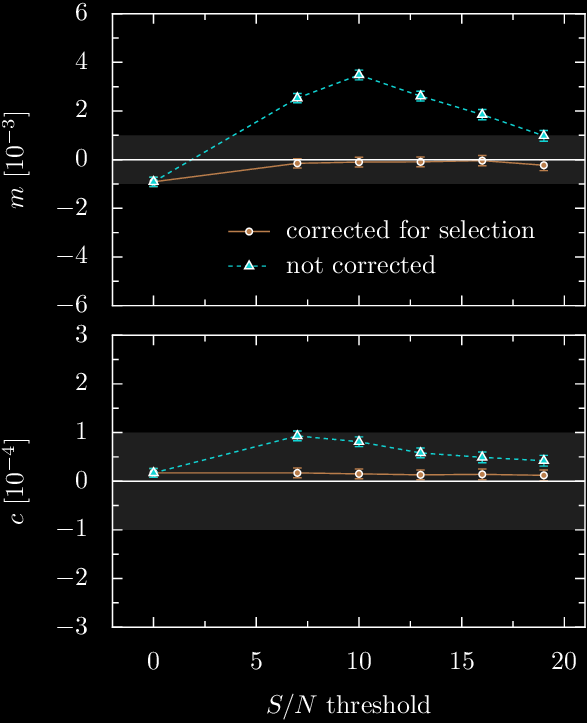
\includegraphics[width=\textwidth]{mc-select-bias-thresh-pyx-inv.png}
                \newline
            \end{center}
        \end{column}
    \end{columns}


}

\frame
{
    \frametitle{\snr\ Ranges}
 

    \begin{columns}
        \begin{column}{0.4\textwidth}
            \begin{itemize}
                \item Select objects with \snr\ within a range.
            \end{itemize}
        \end{column}
        \begin{column}{0.6\textwidth}
            \begin{center}
            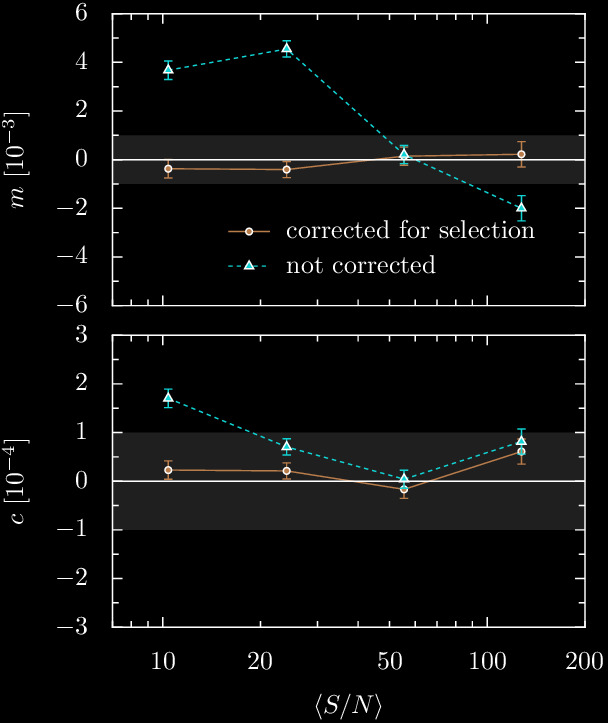
\includegraphics[width=\textwidth]{mc-select-bias-range-pyx-inv.png}
                \newline
            \end{center}
        \end{column}
    \end{columns}


}



\frame
{
    \frametitle{Issues for Metacal and BFD on Real Data}

    \setbeamerfont*{itemize/enumerate body}{size=\large}
    \setbeamerfont*{itemize/enumerate subbody}{parent=itemize/enumerate body}
    \setbeamerfont*{itemize/enumerate subsubbody}{parent=itemize/enumerate body}
 
    \begin{itemize}

        \item For FFTs need to replace bad pixels and masked regions.
            

        \item I've shown that using the best-fit model to replace bad pixels
            works fine as long as
            the mask fraction isn't too high. E.g. epochs in which
            an object is near an edge should be removed.

        
        \item For both Metacal and BFD, to perform null tests, the terms to correct for selection effects
            must be applied

        \item BFD is moment based, can't use uberseg, so need to subtract neighbors
            \begin{itemize}
                \item Use the multi-object fitting catalogs to do this
                \item See my talk at the Science Release sessions on Wed. for details
                    on the multi-object fitting
                \item Might be an improvement over uberseg for any code, but we need
                    to test
            \end{itemize}

    \end{itemize}

}

\frame
{
    \frametitle{Metacal on Y1}

    \setbeamerfont*{itemize/enumerate body}{size=\Large}
    \setbeamerfont*{itemize/enumerate subbody}{parent=itemize/enumerate body}
    \setbeamerfont*{itemize/enumerate subsubbody}{parent=itemize/enumerate body}
 
    \begin{itemize}

        \item I've run on a stripe 82 using the recently released MEDS files

        \item The null tests are not passing yet.
            
        \item We also see issues in the most recent multi-object fitting run; I
            suspect a bug was introduced into the PSF fitting code.

    \end{itemize}

}


\frame
{
    \frametitle{Metacal on Y1}

    \setbeamerfont*{itemize/enumerate body}{size=\large}
    \setbeamerfont*{itemize/enumerate subbody}{parent=itemize/enumerate body}
    \setbeamerfont*{itemize/enumerate subsubbody}{parent=itemize/enumerate body}
 
    \begin{itemize}

        \item Despite the known issues, it would be good to begin testing
            with the catalogs to become familiar with the corrections
            for selection effects.

        \item The recent run is \texttt{us82-001} and is in the ``usual'' place
            \begin{itemize}
                \item \texttt{\$DESDATA/wlpipe/us82-001} at BNL
                \item On the web at
                    \texttt{DESDATA}=\url{http://www.cosmo.bnl.gov/Private/gpfs/workarea/desdata}
            \end{itemize}

        \item Example code for doing null tests, including corrections
            for selections, can be found at
            \begin{itemize}
                \item \url{https://github.com/esheldon/ngmixer\_tests}.
                \item See the \texttt{ngmix\_tests.averaging} module
                \item E.g. \texttt{PSFShapeBinner}
            \end{itemize}
    \end{itemize}

}


\end{document}
